\chapter{Optymalizacja metodą roju cząstek - Particle Swarm Optimizaton} \label{sect:PSO_chapter}

\textit{Streszczenie: W niniejszym rozdziale przedstawiono ideę optymalizacji konstrukcji z wykorzystaniem metaheurystycznego algorytmu Particle Swarm Optimization (PSO). Na początku ogólnie opisano optymalizację w kontekście konstrukcji budowlanych. W dalszej części przytoczono charakterystykę metody PSO w wersji jednokryterialnej. Opisano stworzoną aplikację komputerową do poszukiwania ekstremów metodą PSO i przeprowadzono test na teoretycznym przykładzie funkcji multimodalnej. Następnie opisano rozwinięcie metody do wersji wielokryterialnej, a zaimplementowany algorytm ponownie poddano testom. Na końcu rozdziału przedstawiono rozwijane obecnie systemy optymalizacji wspomagane uczeniem maszynowym.}

\section*{Wprowadzenie}
Znalezienie najlepszej możliwej konfiguracji elementów konstrukcyjnych, zapewniającej poprawne przeniesienie obciążeń statycznych, komfort dynamiczny i najlepiej możliwie tanie, jest zadaniem które na co dzień towarzyszy projektantom mostów. Takie zadanie może kojarzyć się intuicyjnie z pojęciem optymalizacji, czyli wyborem najlepszego z wielu rozwiązań, pozwalającego osiągnąć cel lub kilka celów. W pracy \cite{Szymczak1995} określono następuje elementy, jakie powinno zawierać poprawnie sformułowane zadanie optymalizacji:
\begin{itemize}
	\item kryteria optymalizacji - miarę spełnienia danego celu,
	\item parametry optymalizacji - parametry systemu, które są stałe lub niezależne od projektanta, 
	\item zmienne projektowe - parametry systemu zależne od projektanta,
	\item ograniczenia - elementy określające zakres dopuszczalnych rozwiązań. 
\end{itemize}

Kryterium optymalizacji powinno w sposób wymierny pozwolić na ocenę danego rozwiązania. Przykładem celu przyświecającego projektantowi konstrukcji może być koszt jej wykonania, ilość zużytego materiału czy nakład pracy. Kryterium, które decyduje o wyborze najlepszego rozwiązania nazywane jest funkcją celu. W przypadku istnienia kilku istotnych funkcji celu, mamy do czynienia z optymalizacją wielokryterialną. Zagadnienie polega na minimalizowaniu lub maksymalizowaniu jednocześnie kilku funkcji celu. Jednym z najprostszych rozwiązań tak sformułowanego problemu jest stworzenie jednej, zastępczej funkcji celu. Metoda polega na połączeniu wszystkich kryteriów z zastosowaniem wag dla poszczególnych elementów. Odbywa się to zazwyczaj na zasadzie kombinacji liniowej:
\begin{equation}
	F=\sum_{i=1}^{n}w_i F_i
\end{equation}
gdzie $w_i$ to współczynnik określający wagę kryterium $F_i$. W pracy zostało zastosowane inne rozwiązanie optymalizacji wielokryterialnej. Zagadnienie zostanie omówione teoretycznie w punkcie \ref{sect: multiobjective_opt}. 

W przypadku konstrukcji inżynierskiej, parametry projektowe to przyjęte wartości opisujące ustrój, które nie ulegają zmianie w procesie optymalizacji.  Mogą być one narzucone przez względy technologiczne bądź normowe \parencite{Szymczak1995} lub wynikać z innych założeń projektowych. Z kolei zmienne projektowe $x_i$, jak sama nazwa wskazuje, mogą się zmieniać w procesie optymalizacji i zależą od projektanta. Wybór konkretnych $m$ zmiennych projektowych tworzy rozwiązanie w postaci wektora $\vect{x}=[x_1,x_2,\dots,x_m]^T$, określającego punkt w przestrzeni $m$-wymiarowej.

Z reguły wartości zmiennych projektowych i związane z nimi rezultaty obliczeń muszą spełniać szereg obostrzeń. Wynikają one ponownie ze względów technologicznych, normowych lub innych, zdaniem projektanta, istotnych wartości brzegowych. Z tego powodu, na zmienne projektowe $\vect{x}$ i na inne wartości z nich wynikające narzucone mogą być ograniczenia. Wektor który spełnia wszystkie ograniczenia nazywany jest dopuszczalnym. W analizie konstrukcji budowlanych ograniczeniami mogą być warunki wytrzymałościowe, eksploatacyjne - zarówno statyczne jak i dynamiczne - czy też wymogi stateczności.


\section{\raggedright{Klasyfikacja problemów i metod optymalizacji}}
Wszystkie powyżej opisane składowe definiują problem optymalizacji. Każdy z nich może przyjmować różne postaci, co będzie miało znaczący wpływ przede wszystkim na wybór metody rozwiązania problemu. W pracy \cite{Tesch2016} zaproponowano następującą klasyfikację problemów optymalizacji, uzależnioną od ich elementów charakterystycznych:
\begin{itemize}
	\item Liczba funkcji celu:
	\begin{itemize}
		\item pojedyncza funkcja celu,
		\item wiele funkcji celu.
	\end{itemize}
	\item Liczba ekstremów lokalnych funkcji celu:
	\begin{itemize}
		\item funkcja unimodalna - funkcja jest ciągła i posiada jedno ekstremum w rozpatrywanym przedziale,
		\item funkcja multimodalna - funkcja posiada więcej niż jedno ekstremum lokalne w rozpatrywanym zakresie.
	\end{itemize}
	\item Liniowość funkcji celu:
	\begin{itemize}
		\item problem programowania liniowego - funkcja celu i ograniczenia są liniowe,
		\item problem programowania nieliniowego - funkcja celu lub ograniczenia nie są liniowe.
	\end{itemize}
	\item Rodzaj zmiennych projektowych:
	\begin{itemize}
		\item ciągłe - zmienne projektowe są liczbami rzeczywistymi w zadanym przedziale,
		\item dyskretne - zmienne projektowe są liczbami całkowitymi w zadanym przedziale,
		\item mieszane - w problemie występują zarówno zmienne ciągłe, jak i dyskretne.
	\end{itemize}
\end{itemize}

Klasyfikacje zawarte w klasycznych pozycjach dotyczących optymalizacji podają również ogólny podział ze względu na to czy zmienne projektowe są liczbami, czy funkcjami \parencite{Szymczak1995,Findeisen1980}.

Rodzaj problemu optymalizacji ogranicza wybór metody, którą można użyć do jego rozwiązania. W literaturze algorytmy tradycyjne dzielone są ze względu na sposób przeszukiwania na: analityczne, enumeratywne oraz losowe \parencite{Goldberg1995}. W skrócie, pierwsze opierają się na stworzeniu i rozwiązaniu układu równań, powstałego przez przyrównanie gradientu funkcji celu do zera. Metody te wymagają obliczenia pochodnych funkcji i mają charakter lokalny, szukając optymalnego rozwiązania wokół punktu, a nie w całym dopuszczalnym obszarze. W realnych przypadkach są to trudne do zaakceptowania warunki i metody te mają raczej ograniczony zakres zastosowań. Metody enumeratywne polegają na obliczaniu funkcji celu dla kolejnych rozwiązań dopuszczalnych. W literaturze przedmiotu inną spotykaną nazwą tej metody jest \enquote{systematyczne przeszukiwanie}. Pomimo naturalnego charakteru tej metody i jej prostoty, jest to najmniej efektywna klasa metod, co jest jej główną wadą. Działanie metod losowych jest podobne do systematycznego przeszukiwania, z tą różnicą, że kolejne rozwiązania są dobierane w sposób losowy, a nie uporządkowany. Metody losowe w ogólności nie pozwalają efektywniej uzyskać optymalnego rozwiązania niż enumeratywne. Przedstawione konwencjonalne metody są albo wysoce wyspecjalizowane i swoim zastosowaniem obejmują wąskie spektrum problemów, albo są mało efektywne w szerokim zakresie zastosowań. Znając ograniczenia metod tradycyjnych poszukiwano innych, które dzięki wykorzystaniu maszyn cyfrowych mogą stać się jednocześnie znacznie bardziej efektywne niż metody enumeratywne oraz pozwalają na rozwiązanie znacznie bardziej różnorodnych zadań niż metody analityczne. W odpowiedzi powstały algorytmy, które doboru coraz lepszego rozwiązania dokonują wykorzystując randomizację, ale nie są w zupełności losowe. Są to tak zwane algorytmy heurystyczne i w rozwiniętej wersji metaheurystyczne \parencite{Blum2003}. Cechują się one konkretną strategią, która przewodzi przeszukiwaniu przestrzeni w poszukiwaniu rozwiązania optymalnego. Powinny być uniwersalne i nienakierowane jedynie na konkretny typ problemu. Wykorzystują one doświadczenie powstałe na bazie przeprowadzonych prób i uczą się na ich podstawie, szukając coraz lepszego wyniku. Ponadto, większość algorytmów metaheurystycznych ma charakter globalny i nie ogranicza się do funkcji unimodalnych. Pomimo niewątpliwych zalet, należy pamiętać że algorytmy metaheurystyczne są z natury przybliżone. W związku z tym nie gwarantują, że optymalny wynik zostanie w ogóle odnaleziony. Najbardziej popularne algorytmy metaheurystyczne są inspirowane zachowaniami zaobserwowanymi w naturze \parencite{FisterJr.2013}. Główne mechanizmy ich działania mogą być zaczerpnięte z praw fizyki (np. Algorytm Przeszukiwania Grawitacyjnego \parencite{Rashedi2009}), biologii (np. Algorytmy Genetyczne \parencite{Goldberg1995}) czy inteligencji stadnej (np. Optymizacja Rojem Cząstek \parencite{Clerc2010,Eberhart2001}).
Podsumowując i odwołując się do wyżej przytoczonej klasyfikacji problemów optymalizacji, algorytmy ich rozwiązania  dzielimy według następujących kryteriów \cite{Tesch2016}:
\begin{itemize}
	\item Różniczkowalność funkcji celu:
	\begin{itemize}
		\item wymagające pochodnej - algorytmy tej kategorii wymagają istnienia dwukrotnej pochodnej funkcji celu,
		\item niewymagające pochodnej - algorytmy tej klasy nie wymagają ciągłości funkcji celu oraz jej pochodnej.
	\end{itemize}
	\item Liczba jednocześnie rozważanych rozwiązań:
	\begin{itemize}
		\item jednopunktowe - w jednej chwili rozważane jest jedno rozwiązanie. W kolejnych krokach algorytmu jest ono modyfikowane w celu uzyskania lepszego rozwiązania,
		\item wielopunktowe - jednocześnie odbywa się analiza wielu rozwiązań, które mają wpływ na wynik końcowy.
	\end{itemize}
	\item Mechanizmy losowości:
	\begin{itemize}
		\item deterministyczne - rozwiązania są wyznaczane jedynie na podstawie danych wejściowych i wyznaczonych parametrów,
		\item stochastyczne - zmienne projektowe są wybierane z uwzględnieniem czynnika losowego,
		\item hybrydowe - algorytm zawiera oba mechanizmy wyboru kolejnego rozwiązania.
	\end{itemize}
\end{itemize}

\section{\raggedright{Określenie funkcji celu i wybór metody optymalizacji}}
Wpływ poszczególnych rozwiązań konstrukcyjnych mostów łukowych na jego odpowiedź dynamiczną zalicza się do zagadnień złożonych. 
Pierwszą funkcją celu postawionego problemu może być minimalizacja przyspieszeń pionowych pomostu w trakcie przejazdu. Jest to najczęściej decydujący warunek eksploatacyjny mostu z wymaganych przez normę europejską \parencite{PKNc}. Drugą pożądaną cechą może być poszukiwanie najtańszego obiektu (w uproszczeniu najmniejszej ilości zużytego materiału), przy spełnieniu wszystkich warunków wytrzymałościowych. Wyboru metody optymalizacji użytej w pracy dokonano przez następującą analizę myślową rozpatrywanego zadania. Z uwagi na brak funkcyjnego opisu odpowiedzi dynamicznej modelu numerycznego zaniechano użycia metod analitycznych, wymagających obliczania pochodnych. Dodatkowo problem ma charakter globalny i nie wolno dopuścić do zakończenia poszukiwania w ekstremum lokalnym.  Odrzucono również metody losowe i systematycznego przeszukiwania z uwagi na długotrwałe wyznaczanie funkcji celu i bardzo nieefektywny algorytm. Kolejnym kryterium była uniwersalność algorytmu, ponieważ zaplanowano użycie go w dwóch zupełnie różnych problemach: kalibracji modelu i optymalizacji konstrukcji z punktu widzenia zachowania dynamicznego. Ostatnim kryterium była udokumentowana w literaturze skuteczność metody, w tym wykorzystanie jej w przypadkach analizy i oceny konstrukcji. Powyższe warunki spełniają metody metaheurystyczne. Spośród opisanych w literaturze wybrano metodę optymalizacji rojem cząstek (PSO).
\section{Particle Swarm Optimization} \label{sect:pso_def}
Optymalizacja rojem cząstek \teng{Particle Swarm Optimization (PSO)} jest metaheurystycznym, inspirowanym naturą algorytmem optymalizacji. W bazowej wersji powstał w roku 1995 \parencite{Kennedy1995a,Eberhart1995} i od tamtej pory ulegał wielu modyfikacjom, udoskonaleniom i rozszerzeniom. Metoda zakłada istnienie pewnej populacji - roju, składającego się z $M$ cząstek. Każda cząstka o indeksie $i$ posiada trzy informacje zawarte w wektorach $\vect{x}_i,\vect{v}_i,\vect{p}_i$. Wektory $\vect{x}_i$ i $\vect{p}_i$, każdy o długości $D$, oznaczają punkt w przeszukiwanej przestrzeni $\matr{X}$, gdzie $D$ jest liczbą zmiennych projektowych problemu. $\vect{x}_i$ oznacza aktualną pozycją cząstki w przestrzeni $\matr{X}$. Z kolei $\vect{p}_i$ określa najlepsze dotychczasowe położenie cząstki $i$ \teng{personal best (pbest)}. Jakość położenia określana jest przez wyznaczenie funkcji celu dla danej cząstki. Na przykład zakładając minimalizację, mniejsza wartość funkcji celu jest lepsza od większej. Jeżeli funkcja celu dla nowego położenia cząstki jest lepsza niż zachowana w pamięci (pbest), to wektor $\vect{p}_i$ jest aktualizowany do nowej wartości. $\vect{v}_i$ jest również wektorem o długości $D$ i oznacza różnicę pomiędzy nowym położeniem w chwili $t+1$ i poprzedzającym w chwili $t$:
\begin{equation} \label{eq: pso_position}
	\vect{x}_i^{t+1}=\vect{x}_i^t+\vect{v}_i^{t+1}
\end{equation}
 Jako że wektor $\vect{v}_i$ decyduje o kolejnym położeniu cząstki, nazywany jest wektorem prędkości. Współrzędne wektora $\vect{v}_i$ z kroku $t$ uaktualniane są w kolejnych iteracjach $t+1$ w następujący sposób:
\begin{equation} \label{eq: pso_velocity}
	\vect{v}_{i}^{t+1}=\theta\vect{v}_i^t+\alpha\vect{u}_1^t\circ (\vect{n}_i^t-\vect{x}_i^t)+\beta\vect{u}_2^t\circ(\vect{p}_i^t-\vect{x}_i^t)
\end{equation}
gdzie wektory $\vect{u}_1^t$ i $\vect{u}_2^t$ zawierają zestawy losowych liczb o rozkładzie jednostajnym z zakresu [0,1], ustalonych w chwili czasowej $t$. Symbol $(\circ)$ oznacza iloczyn skalarny. Parametry $\alpha$, $\beta$ i $\theta$ w pierwotnej wersji algorytmu są stałymi. W zależności od zastosowanej topologii roju, $\vect{n}_i$ oznacza najlepsze rozwiązanie $\vect{p}_i$ spośród dostępnych, sąsiednich cząstek. W jednej z najpopularniejszych i najbardziej intuicyjnych wersji stosowana jest topologia \textit{gbest}, w której $\vect{n}_i$ przyjmuje najlepszą wartość $\vect{p}_i$ spośród wszystkich cząstek.
\subsubsection{Parametry algorytmu PSO}
Każdy składnik prędkości spełnia określoną rolę. Pierwszy jest związany z bezwładnością i utrzymuje on bieżącą trajektorię cząstki. Parametr $\theta$ w ogólności zmniejsza prędkość, zapewniając lepszą zbieżność rozwiązania \parencite{Blackwell2019}. Jego wartość może być stała lub zmienna w trakcie analizy. Współczynniki $\alpha$ i $\beta$ odpowiadają za przyspieszenie na bazie odpowiednio własnych i społecznych doświadczeń. 
W pracy \cite{Clerc2002} autorzy wyznaczyli wartości $\theta=0.7968$, $\alpha=1.4962$ i $\beta=1.4962$ jako optymalne z punktu widzenia działania algorytmu. Przyjęcie równości $\alpha=\beta$ oznacza, że na prędkość cząstki równy wpływ mają doświadczenia własne i sąsiadów. Do podobnych rezultatów doszli autorzy pracy \cite{Shi1998}. Z kolei w \cite{Xu2007} podano przykład zmiennego wariantu, gdzie $\theta$ zmniejsza swoją wartość liniowo od 0.9 do 0.4, a parametry $\alpha$ i $\beta$ są stałe i równe 2.0. W \cite{Poli2007} obszernie opisano metody wyznaczania wartości parametrów algorytmu.
\subsubsection{Topologie roju}
Topologa roju odpowiada za zachowanie społeczne cząstek roju.  Określa ona sąsiedztwo, z którym cząstka może się komunikować i wymieniać doświadczeniem. Definiuje również liderów, za którymi podążać będą pozostałe cząstki. Topologie dzielą się na dwie główne grupy: globalne \teng{global best (gbest))} i lokalne \teng{local best (lbest)}. Schemat topologii można przedstawić za pomocą grafów, w których węzły oznaczają cząstki, a krawędzie możliwość komunikacji z inną cząstką (Rys. \ref{fig: pso_topologies}). Trzy najczęściej występujące w literaturze przedmiotu topologie to:
\begin{itemize}
	\item topologia pierścieniowa (Rys. \ref{fig: pso_topologies1}),
	\item topologia pełnego grafu (Rys. \ref{fig: pso_topologies2}),
	\item topologia von Neumanna (Rys. \ref{fig: pso_topologies3}).
\end{itemize}
\begin{figure}[hbt!]
	\centering
	\subfloat[Topologia pierścieniowa]{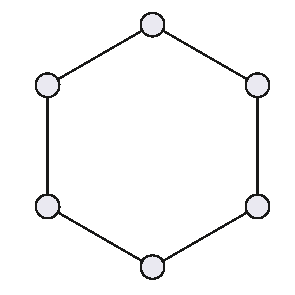
\includegraphics[width=0.3\linewidth]{/PSO/topology/pierscien.pdf} \label{fig: pso_topologies1}}
	\subfloat[Topologia pełnego grafu]{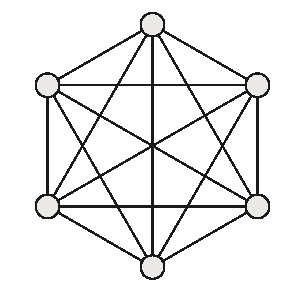
\includegraphics[width=0.3\linewidth]{/PSO/topology/global.pdf} \label{fig: pso_topologies2}}
	\subfloat[Topologia von Neumanna]{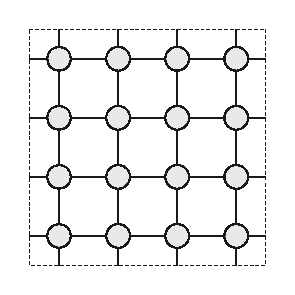
\includegraphics[width=0.3\linewidth]{/PSO/topology/neumann.pdf} \label{fig: pso_topologies3}}
	\captionsetup{justification=centering}
	\caption{Schematy wybranych topologi komunikacji pomiędzy cząstkami w metodzie optymalizacji rojem cząstek}
	\label{fig: pso_topologies}
\end{figure}
Przyjęta topologia roju ma istotny wpływ na zachowanie cząstek i efektywność algorytmu. Topologie należące do rodziny \textit{gbest} osiągają szybciej zbieżność, ale istnieje większe ryzyko na utknięcie w minimum lokalnym, gdy funkcja celu nie jest unimodalna. Innymi słowy przynosi ona precyzyjniejsze rozwiązanie, ale mniej dokładnie przeszukuje obszar. Przy wykorzystaniu rodziny \textit{lbest} efekt jest odwrotny. Ograniczona jest komunikacja jedynie do wąskiego grona sąsiadów, przez co algorytm zbiega do rozwiązania wolniej. Zwiększa to szansę na dokładniejsze przeszukanie obszaru, ale zmniejsza precyzję ostatecznego wyniku. Topologie mogą być również podzielone na statyczne i dynamiczne. Pierwsze utrzymują swoją strukturę przez cały czas wykonywania algorytmu, drugie zmieniają swoje właściwości wraz z postępem obliczeń. Najczęściej w topologiach dynamicznych populacja rozpoczyna od małej liczby sąsiadów, żeby w trakcie wykonywania algorytmu ich liczba stopniowo wzrastała \parencite{Poli2007}. Warto podkreślić, że w klasycznej wersji algorytmu położenie cząstki w przestrzeni $\matr{X}$ nie ma wpływu na początkowy wybór sąsiedztwa zgodnie z założoną topologią.

Jedyną topologią z rodziny \textit{gbest} jest topologia pełnego grafu (Rys. \ref{fig: pso_topologies2}). Każda cząstka może przekazywać informację o najlepszym położeniu do wszystkich innych cząstek. W tym wariancie wektor $\vect{n}_i$ w formule (\ref{eq: pso_velocity}) jest równy dla wszystkich cząstek i odpowiada najlepszemu dotychczasowemu położeniu cząstki w całej populacji. Z kolei historycznie pierwszą i najprostszą topologią \textit{lbest} jest topologia pierścieniowa (Rys. \ref{fig: pso_topologies1}). Komunikacja w niej jest zapewnione jedynie pomiędzy najbliższymi sąsiadami: cząstka o indeksie $i$ wymienia informację o najlepszym położeniu jedynie z cząstkami o indeksach $i-1$ i $i+1$. Trzecia wymieniona topologia von Neumanna należy również do rodziny \textit{lbest}, ale reprezentuje kompromis pomiędzy przypadkami skrajnymi: topologią pierścieniową i pełnego grafu (Rys. \ref{fig: pso_topologies3}). Pozwala ona na wymianę informacji z czterema sąsiadami. Autorzy w pracy \parencite{Kennedy2002} wykonali szereg testów obliczeniowych dla zróżnicowanych problemów i dla wielu topologii. W tym teście topologia von Neumanna otrzymała najwyższą sumaryczną notę i jest opisana jako najbardziej uniwersalna. Obszerne porównanie topologii wraz z historycznym opisem ich powstania i efektywnością zostało zawarte w pracy \parencite{Blackwell2019}.

\subsubsection{Generacja populacji}
Początkowa populacja roju jest rozmieszczana w $D$-wymiarowej przestrzeni rozwiązań $\matr{X}$. Przyjęcie właściwej liczby cząstek roju nie jest kwestią ściśle określoną. W tekście \cite{Piotrowski2020} pokazano przeprowadzone obszerne studium dotyczące przyjęcia wstępnej liczebności populacji. Posłużono się kilkudziesięcioma rzeczywistymi i testowymi problemami optymalizacji i oceniono 8 różnych wersji algorytmu. Na bazie analizy statystycznej stwierdzono, że klasycznie zalecanie przyjęcia od 20 do 50 cząstek \parencite{Liang2006,Chen2012,Harrison2018} jest w przypadku wielu rzeczywistych problemów niewystarczające. Taka liczba sprawdza się jedynie dla stosunkowo prostych problemów unimodalnych. Dla złożonych zagadnień i rozbudowanych wersji algorytmu (podobnych do opisanego w niniejszej pracy), autorzy podali poprawny zakres liczebności roju od 70 do 500 cząstek. Jednocześnie sformułowano również generalną wskazówkę, że dla wszystkich wariantów algorytmu PSO bezpiecznym rozwiązaniem jest przyjęcie od 70 do 100 cząstek. Liczebność populacji w trakcie całej analizy jest zazwyczaj stała, chociaż istnieją modyfikacje algorytmu, które pozwalają na dodawanie cząstek w trakcie przebiegu optymalizacji.

\begin{figure}[hbt!]
	\centering
	\subfloat[]{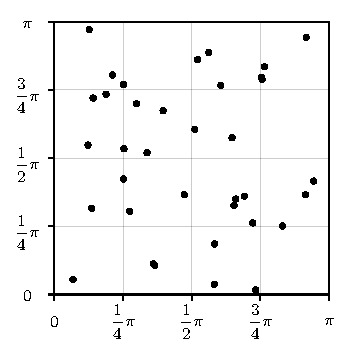
\includegraphics[width=0.45\linewidth]{/PSO/population/fig_population_random1.pdf} \label{fig: pso_gen_rand_1}}
	\subfloat[]{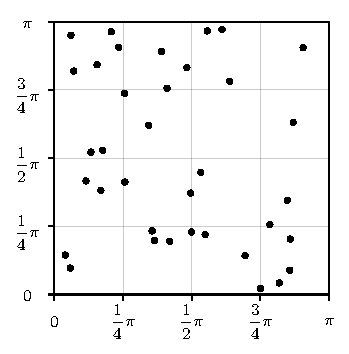
\includegraphics[width=0.45\linewidth]{/PSO/population/fig_population_random2.pdf} \label{fig: pso_gen_rand_2}}\\
	\subfloat[]{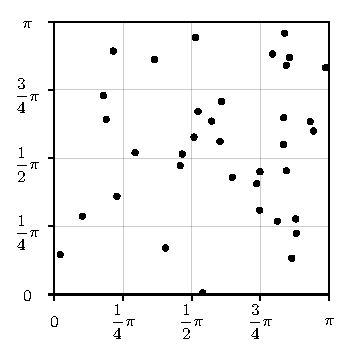
\includegraphics[width=0.45\linewidth]{/PSO/population/fig_population_random3.pdf} \label{fig: pso_gen_rand_3}}
	\subfloat[]{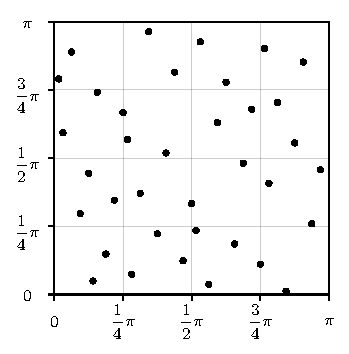
\includegraphics[width=0.45\linewidth]{/PSO/population/fig_population_halton.pdf}  \label{fig: pso_gen_halton}}
	\captionsetup{justification=centering}
	\caption{Przykłady rozkładu wygenerowanych populacji cząstek: (a)-(c) generacja losowa, (d) generacja z wykorzystaniem sekwencji Haltona}
	\label{fig: pso_gen_expl}
\end{figure}

Rozwiązania realnych zagadnień inżynierskich zazwyczaj cechują pewne ograniczenia, które przekładają się na dopuszczalny zakres zmiennych projektowych. Jeżeli zestaw minimalnych, dopuszczalnych wartości zmiennych projektowych zebrany zostanie w wektorze $\vect{x}_{min}$, a maksymalnych w wektorze $\vect{x}_{max}$, to możliwe jest określenie hiperprostokąta o wierzchołkach $(\vect{x}_{min},\vect{x}_{max})$. Początkowe położenie cząstek odbywa się przez dobranie współrzędnych wektorów rozwiązań $x_i$, tak aby wszystkie cząstki znalazły się wewnątrz hiperprostokąta $(\vect{x}_{min},\vect{x}_{max})$. Pozycje początkowe mogą być wybierane przez użytkownika bądź losowane wewnątrz przestrzeni dopuszczalnych rozwiązań. Zakładając niewielką populację roju, istnieje spora szansa, że losowanie o jednorodnym rozkładzie nie zagwarantuje równomiernego pokrycia przestrzeni. Z tego powodu do generacji początkowej populacji niekiedy stosowane są deterministyczne algorytmy, które pozwalają uzyskać rozkład do złudzenia przypominający losowy, ale jednocześnie zapewniające równomierną dystrybucję w przestrzeni \parencite{Saliby2002}. Jedną z takich metod jest wykorzystanie sekwencji Haltona \parencite{Tesch2016}. Na rysunku \ref{fig: pso_gen_expl} pokazano przykłady rozkładu początkowych położeń 36 cząstek w przestrzeni dwuwymiarowej. Trzykrotnie wylosowano populację za pomocą generatora pseudolosowego (Rys. \ref{fig: pso_gen_rand_1}$-$\ref{fig: pso_gen_rand_3}). Dla kontrastu przedstawiono punkty wygenerowane za pomocą sekwencji Haltona (Rys. \ref{fig: pso_gen_halton}). W każdej z losowo wybranych populacji widoczne są obszary, które są gęsto pokryte i takie, w którym nie znajduje się żadna cząstka. Przy wykorzystaniu sekwencji Haltona przestrzeń jest pokryta znacznie bardziej równomiernie. Problem staje się tym bardziej istotny kiedy dotyczy małych populacji. Jeśli wyznaczenie wartości funkcji celu jest bardzo kosztowne czasowe i zadanie jest wielowymiarowe, to równomierny rozkład początkowy cząstek w przestrzeni zmiennych projektowych ułatwia znalezienie ekstremum globalnego w mniejszej liczbie iteracji.

%
\subsubsection{Warunki brzegowe}
Jak wspomniano wcześniej początkowa populacja roju jest losowana wewnątrz przestrzeni dopuszczalnych rozwiązań. Następnie wykorzystana jest inteligencja roju do przeszukania przestrzeni w celu znalezienia ekstremum globalnego. W kolejnych iteracjach położenie cząstek zmieniane jest zgodnie z zależnościami (\ref{eq: pso_velocity}) i (\ref{eq: pso_position}). W trakcie obliczeń, w oryginalnej wersji algorytmu, użytkownik nie ingeruje w proces przemieszczania się cząstek. Istnieje więc możliwość, że wyznaczona prędkość wyprowadzi cząstkę poza obszar dopuszczalnych rozwiązań. Jest to szczególnie prawdopodobne kiedy ekstremum globalne znajduje się w pobliżu granicy rozwiązań dopuszczalnych \parencite{Xu2007}. Jeśli cząstka wyjdzie poza zakres dopuszczalnych rozwiązań, to jej wartość jest nieistotna (błędna) dla projektanta i nie powinna wpływać na wynik końcowy optymalizacji. Jednym z rozwiązań jest obciążenie takiej cząstki karą. Do wartości funkcji celu dodawana jest liczba, która drastycznie oddali wynik od najlepszego rezultatu (dla minimalizacji zwiększenie wyniku, a dla maksymalizacji pomniejszenie). 
Aby zniwelować efekt ucieczki cząstek z obszaru dopuszczalnego, zastosowana może być prędkość maksymalna $\vect{v}_{max}$ połączona ze współczynnikiem zaciskania \parencite{Eberhart2001a}. Zalecana prędkość maksymalna może być powiązana z rozpiętością zakresu zmiennych projektowych $\vect{v}_{max}=\vect{x}_{max}-\vect{x}_{min}$. Drugim stosowanym zabiegiem jest zdefiniowanie warunków brzegowych. Modyfikują one parametry cząstki (położenie lub prędkość), jeżeli znajdzie się ona poza obszarem dopuszczalnych rozwiązań. W literaturze spotykane są cztery podstawowe rodzaje warunków brzegowych: absorbujący \teng{absorbing wall}, odbijający \teng{reflecting wall}, tłumiący \teng{damping wall} i niewidoczny \teng{invisible wall} \parencite{Robinson2004,Huang2005}. Efekt poszczególnych warunków brzegowych, przy przekroczeniu przez cząstkę granicy danego wymiaru, jest następujący:
\begin{itemize}
	\item absorbujący - cząstka jest zatrzymywana na granicy, a składowa wektora prędkości w danym wymiarze jest zerowana,
	\item odbijający -  cząstka jest zatrzymywana na granicy, a znak składowej prędkości w danym wymiarze jest odwracany,
	\item tłumiący - cząstka jest zatrzymywana na granicy, znak składowej prędkości w danym wymiarze jest odwracany, a wartość składowej jest pomniejszana przez losowy mnożnik z zakresu $(0,1)$,
	\item niewidoczny - cząstka nie jest zatrzymywana na granicy, a wektor prędkości nie zmienia swojej definicji. Wartość funkcji celu nie jest wyznaczana.
\end{itemize} 

Na rysunku \ref{fig: pso_bounds_types} pokazano efekt oddziaływania każdego z wymienionych warunków brzegowych na cząstkę znajdującą się w przestrzeni 2D.  W pracy \parencite{Xu2007} zbadano dodatkowe warianty warunków brzegowych, opierające się na powyższych założeniach, ale niewymuszające zmiany położenia cząstki. Modyfikacji ulegała jedynie prędkość. Autorzy podanych prac zgodnie określają warunek tłumiący jako najbardziej uniwersalny, a warunek niewidoczny jako najwydajniejszy w większości problemów.

\begin{figure}[hbt!]
	\centering
	\subfloat[Absorbujący]{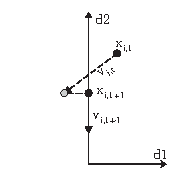
\includegraphics[height=4cm, trim=25 5 0 5, clip]{/PSO/bounds/absorb.pdf} \label{fig: pso_bounds_abs}}
	\subfloat[Odbijający]{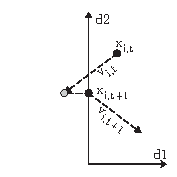
\includegraphics[height=4cm, trim=20 5 0 5, clip]{/PSO/bounds/refl.pdf} \label{fig: pso_bounds_refl}}
	\subfloat[Tłumiący]{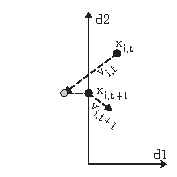
\includegraphics[height=4cm, trim=20 5 0 5, clip]{/PSO/bounds/damp.pdf} \label{fig: pso_bounds_damp}}
	\subfloat[Niewidoczny]{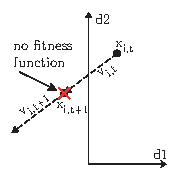
\includegraphics[height=4cm, trim=0 5 5 5, clip]{/PSO/bounds/inv.pdf} \label{fig: pso_bounds_inv}}
	\captionsetup{justification=centering}
	\caption{Rodzaje warunków brzegowych wpływające na zachowanie cząstki wychodzącej poza zakres rozwiązań dopuszczalnych}
	\label{fig: pso_bounds_types}
\end{figure}


\subsubsection{Warunki zakończenia}
Algorytm PSO z każdą kolejną iteracją aktualizuje położenie cząstek i pamięć roju. Zakończenie przeszukiwania przestrzeni może być wymuszone na różne sposoby. Najprostszą metodą jest określenie maksymalnej liczby aktualizacji roju, po której poszukiwanie zostanie zakończone. W tym przypadku na wstępie wiadomym jest ile iteracji zostanie wykonanych i przy znajomości czasu potrzebnego na oszacowanie wartości funkcji celu możliwe jest określenie długości całego procesu optymalizacji. Podstawową wadą tego kryterium jest to, że nie odnosi się w żaden sposób do jakości rozwiązania w ciągu trwania obliczeń. W pracy \parencite{Zielinski2007} przedstawiono zestaw innych warunków zakończenia, które uwzględniają zachowanie roju w trakcie poszukiwań. Wyróżniono następujące kryteria wpływające na zakończenie algorytmu:
\begin{itemize}
	\item kryterium postępu - optymalizacja jest zatrzymana kiedy w określonej liczbie kolejnych iteracji nie nastąpi znaczące polepszenie ekstremum globalnego,
	\item kryterium ruchu - optymalizacja jest zatrzymywana kiedy położenie bieżącego ekstremum globalnego (w przestrzeni zmiennych projektowych) nie zmienia się istotnie w określonej liczbie kolejnych iteracji,
	\item kryterium dystrybucji populacji - optymalizacja jest zatrzymywana kiedy cząstki zgrupują się w jednym miejscu. Dystrybucja może być mierzona między innymi przez odchylenie standardowe położenia populacji, maksymalny dystans między cząstkami lub rozmiar roju mierzony przez długość boków hiperprostokąta, w którym w całości się mieści.  
	\item kryterium prędkości - optymalizacja jest zatrzymywana kiedy prędkość cząstek roju spadnie poniżej wartości minimalnej i nie wzrośnie przez określoną liczbę kolejnych iteracji. 
\end{itemize}
Wszystkie powyższe warunki mogą być łączone i użyte wedle potrzeb w zależności od specyfiki problemu optymalizacji. W pracy \cite{Banach2017} autor określił kryterium prędkości jako najbardziej uniwersalne, ponieważ nie dotyczy położenia cząstek roju i nie zależy od rozwiązywanego problemu optymalizacji. Uzasadnił że nie wymaga ono znajomości wartości progowych dla najczęściej nieznanej ekstremalnej wartości funkcji celu, a także nie wymaga by wszystkie cząstki zbiegły w tym samym miejscu w przestrzeni zmiennych projektowych.
\subsubsection{Schemat blokowy algorytmu}
Podsumowując wszystkie omówione wyżej aspekty, algorytm podstawowej wersji metody optymalizacji rojem cząstek (PSO) przedstawiono na rysunku \ref{fig: pso_single_algorith}.

\begin{figure}[H]
	\centering
	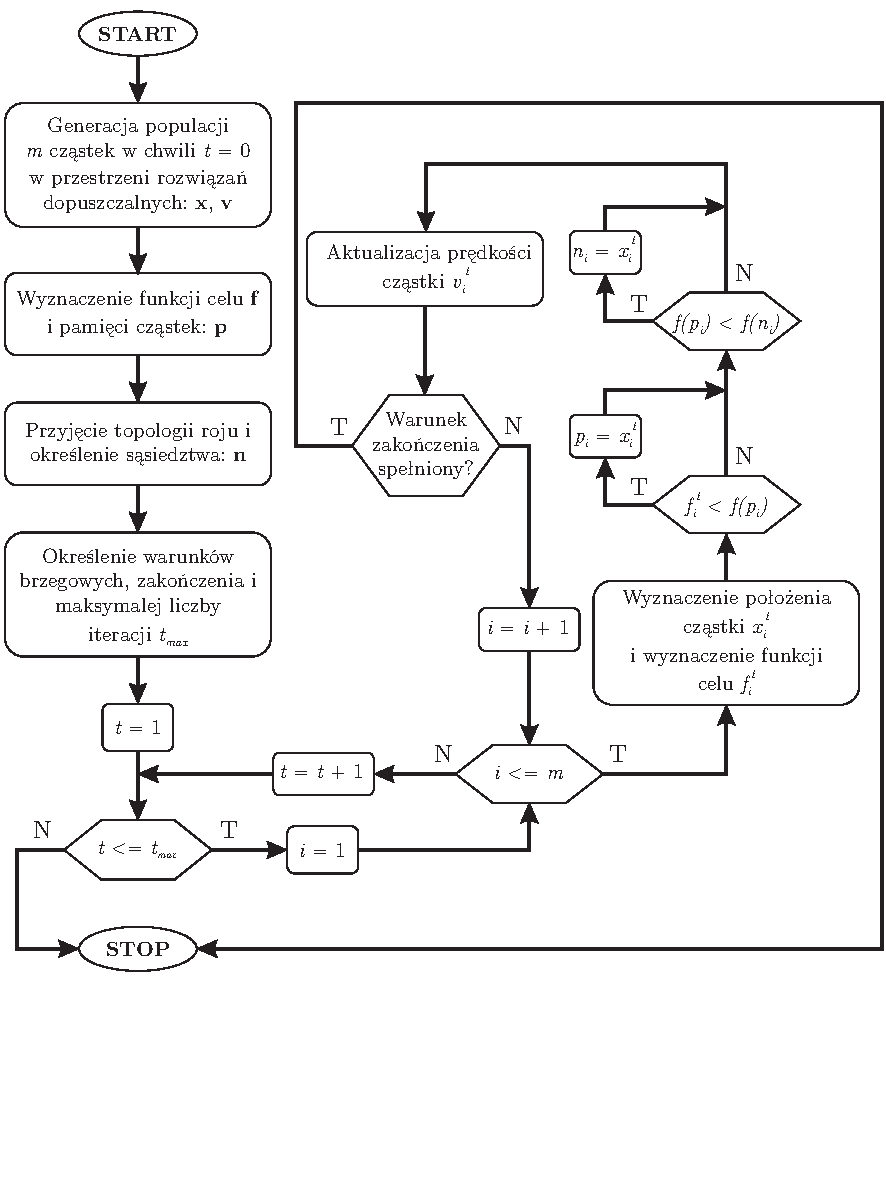
\includegraphics[trim= 0 100 0 0, clip, width=0.9\linewidth]{/PSO/algorithm/algorithm2.pdf} 
	\captionsetup{justification=centering}
	\caption{Podstawowy algorytm optymalizacji jednokryterialnej metodą roju cząstek PSO. Przypadek minimalizacji}
	\label{fig: pso_single_algorith}
\end{figure}


\subsection{Zastosowania optymalizacji algorytmem PSO}
W literaturze udokumentowano wiele zastosowań algorytmu PSO przy rozwiązywaniu rzeczywistych problemów optymalizacji. Dotyczą one różnych dziedzin nauki: inżynierii, informatyki i telekomunikacji, ekonomii czy medycyny. Przeglądowe artykuły podsumowujące prace związane z PSO \cite{Atyabi2011,CoelloCoello2006,Lalwani2013} wskazują na ciągły wzrost liczby publikacji traktujących o wykorzystaniu algorytmów PSO. Nie sposób przytoczyć je wszystkie, dlatego wymieniono kilka dotyczących problemów inżynierii lądowej. W \cite{Hughes2018} zastosowano PSO w procesie kalibracji urządzenia kontrolującego odpowiedź dynamiczną mostu autostradowego. W pracach \cite{Seyedpoor2011,Kang2012,Wei2018} wykorzystano optymalizację rojem cząstek przy detekcji uszkodzeń konstrukcji. Ciekawe zastosowanie algorytmu przedstawiono w \cite{Tran-Ngoc2018,Qin2018}, gdzie zastosowano algorytm optymalizacji przy kalibracji modelu numerycznego mostu. Z kolei w \cite{Dan2015} użyto PSO do identyfikacji siły w wantach mostu podwieszonego, przy braku możliwości stosowania klasycznych rozwiązań z uwagi na dołączone tłumiki.

\subsection{Przykład teoretyczny} \label{sect: pso_single_teor_exampl}
W celu weryfikacji stosowanej metody przygotowano przykład teoretyczny. Zastosowano wariant minimalizacji wartości funkcji celu za pomocą metody PSO. Zaimplementowano algorytm PSO w języku Python. Do testu wybrano funkcję multimodalną przedstawioną w pracy \parencite{Tesch2016} i daną wzorem:
\begin{equation} \label{eq: pso_test_func}
	f(x,y) = -5\sin{x}\sin{y}-5\sin{7x}\sin{7y}
\end{equation}
gdzie $x$, $y$ tworzą wektor zmiennych projektowych, a wartość funkcji $f(x,y)$ jest funkcją celu. Wykres funkcji w przestrzeni 3D przedstawiono na rysunku \ref{fig: pso_example_function}. Podobnie jak w pracy źródłowej przedział dopuszczalny dla każdej zmiennej projektowej to $[0,\pi]$. Wartość minimalna funkcji celu w tej dziedzinie jest znana i wynosi $f_{\text{min}}=-6$ dla punktu $(x,y)=(\frac{\pi}{2},\frac{\pi}{2})$.
\begin{figure}[h]
	\centering
	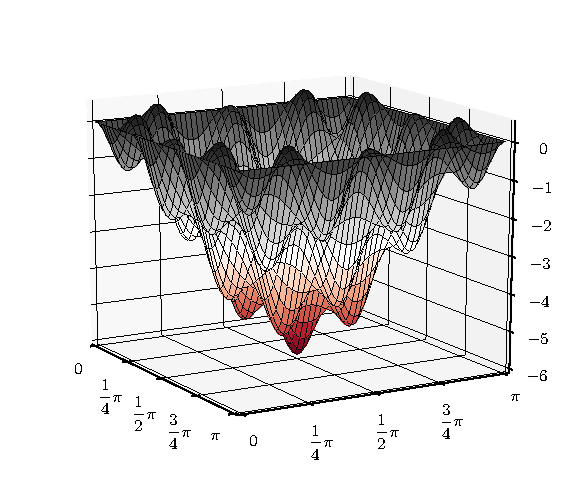
\includegraphics[trim= 0 0 0 20, clip,width=0.7\linewidth]{/PSO/testfunct/fig_3dplot_19_09_18.pdf} 
	\captionsetup{justification=centering}
	\caption{Wizualizacja funkcji testowej w przestrzeni trójwymiarowej}
	\label{fig: pso_example_function}
\end{figure}

Wygenerowano populację złożoną z 20 cząstek. Do generacji użyto wariant korzystający z sekwencji Haltona. Z uwagi na multimodalność funkcji celu zastosowano topologię von Neumanna z rodziny \textit{lbest}. Warunki brzegowe przyjęto typu niewidocznego. Parametry wektora prędkości (\ref{eq: pso_velocity}) ustawiono domyślnie równe: $\theta=0.7968$, $\alpha=1.4962$ oraz $\beta=1.4962$. Zatrzymanie algorytmu nastąpiło po wykonaniu założonej liczby aktualizacji całego roju równej 25. W konsekwencji całkowita liczba ewaluacji wartości funkcji celu wyniosła $25\cdot20=500$. Na rysunku \ref{fig: pso_convergence_plot} zaprezentowano diagram poprawy najlepszego rozwiązania znalezionego przez rój. Na rysunku \ref{fig: pso_test_func_all} pokazano 6 wybranych etapów z całego procesu poszukiwania minimum funkcji. Ostateczna znaleziona wartość minimum globalnego wyniosła $f_{\text{min,25}}=-5.99$. Wartość ta została osiągnięta po około 400 ewaluacjach funkcji i jest bardzo bliska obliczonemu analitycznie minimum globalnemu. Warto nadmienić, że już po 215 ewaluacjach odnalezione zostało rozwiązanie o wartości funkcji celu wynoszącej $f=-5.98$. Wizualizacja położenia cząstek roju w kolejnych iteracjach pokazuje, że wraz z postępem algorytmu cząstki z rozproszonego układu skupiają się konsekwentnie wokół lidera. Topologia von Neumanna z reguły spowalnia ten proces. Z jednej strony opóźnia to znalezienie precyzyjnego rozwiązania, ale jednocześnie obszar dopuszczalny jest przeszukany dokładniej. Na kolejnych grafikach z przebiegu procesu widać, że pomimo znalezienia punktu bliskiego teoretycznemu minimum globalnemu (Rys. \ref{fig: pso_test_func_2}), wciąż pozostają cząstki, które eksplorują cały obszar. Na podstawie powyższego testu uznano, że zaimplementowany algorytm PSO działa poprawnie.
\begin{figure}[hbt!]
	\centering
	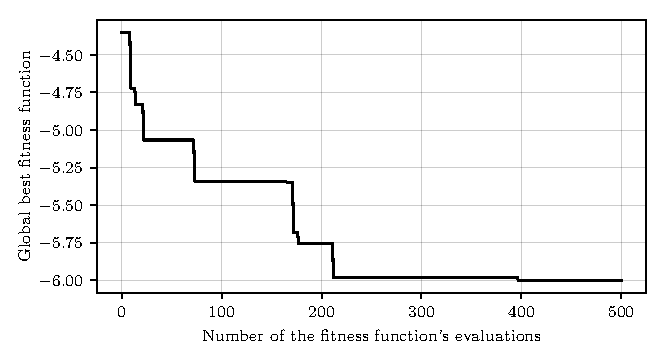
\includegraphics[trim=0 5 0 5, clip,width=0.8\linewidth]{/PSO/testfunct/fig_convergence11_30_59.pdf} 
	\captionsetup{justification=centering}
	\caption{Diagram postępu roju cząstek w poszukiwaniu minimum globalnego funkcji testowej}
	\label{fig: pso_convergence_plot} 
\end{figure}

\begin{figure}[hbt!]
	\centering
	\subfloat[$f_{\text{min,0}}=-4.38$]{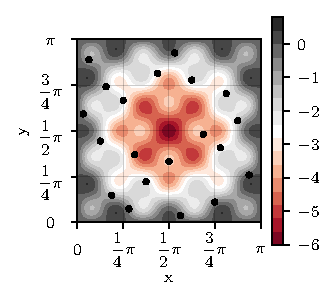
\includegraphics[trim=8 10 5 10, clip,width=0.33\linewidth]{/PSO/testfunct/fig_population_11_30_23.pdf} \label{fig: pso_test_func_1}}
	\subfloat[$f_{\text{min,5}}=-5.34$]{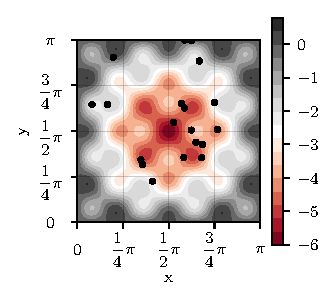
\includegraphics[trim=8 10 5 10, clip,width=0.33\linewidth]{/PSO/testfunct/fig_04_00.pdf} \label{fig: pso_test_func_2}}
	\subfloat[$f_{\text{min,10}}=-5.75$]{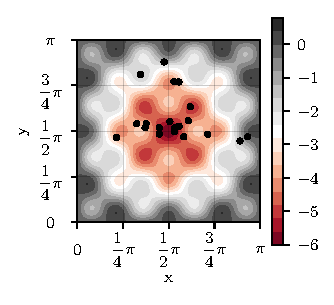
\includegraphics[trim=8 10 5 10, clip,width=0.33\linewidth]{/PSO/testfunct/fig_09_00.pdf} \label{fig: pso_test_func_3}}\\
	\subfloat[$f_{\text{min,15}}=-5.98$]{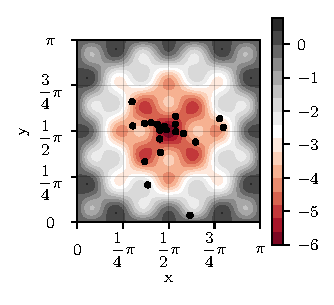
\includegraphics[trim=8 10 5 10, clip,width=0.33\linewidth]{/PSO/testfunct/fig_14_00.pdf} \label{fig: pso_test_func_4}}
	\subfloat[$f_{\text{min,20}}=-5.99$]{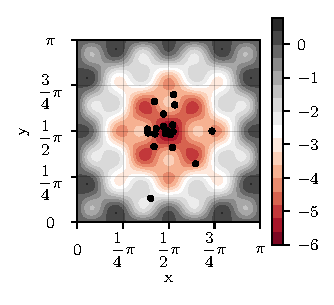
\includegraphics[trim=8 10 5 10, clip,width=0.33\linewidth]{/PSO/testfunct/fig_19_00.pdf} \label{fig: pso_test_func_5}}
	\subfloat[$f_{\text{min,25}}=-5.99$]{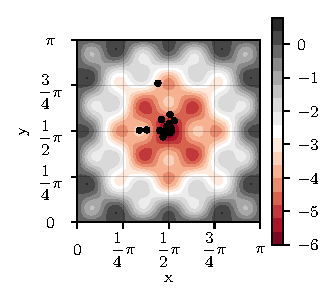
\includegraphics[trim=8 10 5 10, clip,width=0.33\linewidth]{/PSO/testfunct/fig_24_00.pdf} \label{fig: pso_test_func_6}}
	\captionsetup{justification=centering}
	\caption{Etapy rozwiązania testowego problemu optymalizacji dwuwymiarowej za pomocą roju cząstek. Minimum globalne znalezione przez rój oznaczono przez $f_{\text{min},t}$, gdzie indeks $t$ oznacza liczbę pełnych aktualizacji położenia roju. Za pomocą izomapy pokazano wartość funkcji celu na płaszczyźnie}
	\label{fig: pso_test_func_all}
\end{figure}



\section{Optymalizacja wielokryterialna} \label{sect: multiobjective_opt}
Jak wspomniano we wstępie rozdziału, rzeczywiste problemy inżynierskie rzadko sprowadzają się do jednego kryterium, którego optymalizacja dostarcza bezkompromisowo jedno, idealne rozwiązanie. Najczęściej występuje kilka istotnych kryteriów stojących ze sobą w kontrze, których osiągnięcie jest niemożliwe dla tych samych wartości zmiennych projektowych. Przykładem dla konstrukcji budowlanych może być koszt wykonania i szeroko pojęte bezpieczeństwo. Pierwsze z kryteriów zazwyczaj jest minimalizowane, a drugie maksymalizowane. Niestety występuje między nimi konflikt. Z reguły prawidłowe zużycie większej ilości materiału zwiększa koszt i jednocześnie bezpieczeństwo. Przeciwnie, mniejszy koszt poniesiony na budowę z reguły zmniejsza jej bezpieczeństwo. Osiągnięcie jednocześnie minimalnego kosztu i maksymalnego bezpieczeństwa jest więc niemożliwe i trzeba zgodzić się na kompromis. Jedna z metod radzenia sobie w takich przypadkach została już opisana i polega na liniowej kombinacji kryteriów, sprowadzając problem optymalizacji \textit{de facto} do jednej funkcji celu. Wadą tego rozwiązania jest konieczność ustalenia skali ważności poszczególnych kryteriów jeszcze przed rozpoczęciem optymalizacji. Poza koniecznością ustalenia wag składników sumy, niekiedy trudno ustalić związki między zmiennymi projektowymi i kryteriami, a następnie sprowadzić wszystkie kryteria do jednego porównawczego, jakim jest na przykład koszt wykonania lub ilość materiału \parencite{Szymczak1995}. Inną metodą jest rozwiązanie problemu optymalizacji jako zadania wielokryterialnego. Polega ona na jednoczesnej minimalizacji lub maksymalizacji więcej niż jednej funkcji celu. W konsekwencji zamiast pojedynczego optymalnego rozwiązania - jak to ma miejsce w przypadku optymalizacji jednokryterialnej - otrzymywany jest zestaw wielu rozwiązań. Każde z tych rozwiązań jest optymalne, ponieważ nie jest możliwe polepszenie jednego z kryteriów, bez osłabienia pozostałych. Jest to tak zwany zbiór Pareto, zawierający rozwiązania niezdominowane. Do wytłumaczenia powyższego zdania niezbędne jest przytoczenie kilku formalnych definicji zaczerpniętych z pracy \parencite{CoelloCoello2006}. 

Rozpatrzmy problem minimalizacji zestawu $k$ funkcji celu $\vect{f}(\vect{x})$ zależnych od $D$-wymiarowego wektora zmiennych projektowych $\vect{x}$:
\begin{equation}
	\vect{f}(\vect{x})=[f_1(\vect{x}),f_2(\vect{x}),\dots,f_k(\vect{x})] \qquad f_i:\mathbb{R}^D\rightarrow \mathbb{R},\quad i=1,\dots,k
\end{equation}
Dodatkowo niech zbiór $\mathcal{N}$ jest zbiorem liczba naturalnych takich, że $\mathcal{N}=[1,\dots,D]$.
\begin{definition}[Dominacja Pareto]
Niech dwa wektory $\vect{x}_1, \vect{x}_2$ są zdefiniowane w przestrzeni $\mathbb{R}^D$. W przypadku minimalizacji, wektor $\vect{x}_1$ dominuje nad wektorem $\vect{x}_2$, jeżeli każdy element $x_{1,i}$ jest nie większy niż $x_{2,i}$ dla $i\in \mathcal{N}$ i istnieje taki element $x_{1,j}$, że $x_{1,j}$ jest mniejszy niż $x_{2,j}$ dla $j\in\mathcal{N}$. Dominację wektora $\vect{x}_1$ nad $\vect{x}_2$ oznacza się przez $\vect{x}_1\prec\vect{x}_2$.
\begin{equation}
	\bigforall_{i\in\mathcal{N}} x_{1,i}\le x_{2,i} \land \bigexists_{j\in\mathcal{N}} x_{1,j}<x_{2,j}
\end{equation}
\end{definition}


Należy jednak nadmienić, że w kontekście optymalizacji wielokryterialnej, pojęcie dominacji dotyczy przestrzeni funkcji celu, a nie przestrzeni rozwiązań. Optymalny zbiór Pareto zawiera wszystkie rozwiązania $\vect{x}$ w przestrzeni $\mathbb{R}^D$, dla których nie istnieje inny punkt dominujący w przestrzeni funkcji celu $\mathbb{R}^k$. Graficzną prezentację pojęć dominacji w sensie Pareto i Frontu Pareto przedstawiono na rysunku \ref{fig: PSO_pareto_visualization} dla przestrzeni dwóch funkcji celu.

\begin{definition}[Zbiór Pareto]
	Zbiór Pareto $\mathcal{PS}$ rozwiązania, jest zbiorem punktów $\vect{x}$, dla których wśród zestawu rozwiązań dopuszczalnych $\vect{\Omega}$ nie istnieje inny punkt dominujący ze względu na wartość funkcji $\vect{f}(\vect{x})$.
	\begin{equation}
		\mathcal{PS} = \bigg\{ 
		\vect{x}_j \in \vect{\Omega}: 
		\bigforall_{\vect{x}\in\vect{\Omega}} \bigg( 
		\bigexists_{i\in\mathcal{N}} f_i(\vect{x})>f_i(\vect{x_j}) \vee
		\bigforall_{i\in\mathcal{N}} f_i(\vect{x})\ge f_i(\vect{x_j})
		\bigg) \bigg\}   
	\end{equation}
\end{definition}
\begin{definition}[Front Pareto]
	Front Pareto $\mathcal{PF}$ jest zbiorem punktów $\vect{f}(\vect{x})$ w przestrzeni funkcji celu, wyznaczonych dla punktów $\vect{x}$ należących do Zbioru Pareto $\mathcal{PS}$.
	\begin{equation}
		\mathcal{PF} = \big\{ \vect{f}(\vect{x}) \in \mathbb{R}^k: \vect{x}\in \mathcal{PS} \big\}  
	\end{equation}
\end{definition}

W literaturze znaleźć można również definicję $\epsilon$-dominacji w sensie Pareto \parencite{Zuluaga2016}. Polega ona na rozluźnieniu warunku klasycznej dominacji przez dodatnie tolerancji. Akceptowalne różnice zdefiniowane są w wektorze tolerancji $\vect{\epsilon}=[\epsilon_1,\epsilon_2,\dots,k]$, gdzie $\epsilon_i>0$ dla $i=1,2\dots,k$. Wizualizację graficzną Frontu Pareto z zastosowaniem $\epsilon$-dominacji przedstawiono na rysunku \ref{fig: PSO_eps_pareto_visualizationc}.

\begin{definition}[$\epsilon$-dominacja Pareto]
	Niech dwa wektory $\vect{x}_1, \vect{x}_2$ są zdefiniowane w przestrzeni $\mathbb{R}^D$. W przypadku minimalizacji, wektor $\vect{x}_1$ $\epsilon$-dominuje nad wektorem $\vect{x}_2$, jeżeli każdy element $x_{1,i}$ pomniejszony o tolerancję $\epsilon_i$ jest nie większy niż $x_{2,i}$ dla $i\in \mathcal{N}$ i istnieje taki element $x_{1,j}$, że $x_{1,j}-\epsilon_j$ jest mniejszy niż $x_{2,j}$ dla $j\in\mathcal{N}$. $\epsilon$-dominację wektora $\vect{x}_1$ nad $\vect{x}_2$ oznacza się przez $\vect{x}_1\prec_\epsilon\vect{x}_2$.
	\begin{equation}
		\bigforall_{i\in\mathcal{N}} x_{1,i}-\epsilon_i\le x_{2,i} \land \bigexists_{j\in\mathcal{N}} x_{1,j}-\epsilon_j<x_{2,j}
	\end{equation}
\end{definition}


\begin{figure}[hbt!]
	\centering
	\subfloat[Dominacja]{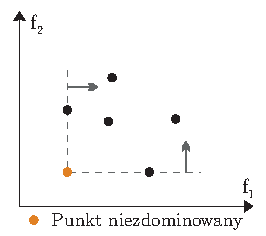
\includegraphics[]{/PSO/pareto/nondominated.pdf} \label{fig: PSO_pareto_visualizationa}}
	\subfloat[Front Pareto]{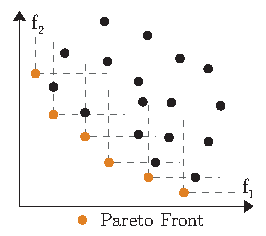
\includegraphics[]{/PSO/pareto/pareto_front.pdf} \label{fig: PSO_pareto_visualizationb}}
	\subfloat[$\epsilon$-Front Pareto]{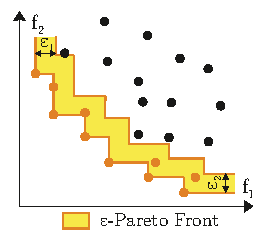
\includegraphics[]{/PSO/pareto/eps_pareto_front.pdf} \label{fig: PSO_eps_pareto_visualizationc}}
	\captionsetup{justification=centering}
	\caption{Wizualizacja definicji dominacji, Frontu Pareto i Frontu Pareto z zastosowaniem $\epsilon$-dominacji}
	\label{fig: PSO_pareto_visualization}
\end{figure}

Przyjmując powyższe definicje optymalizacja wielokryterialna sprowadza się więc do znalezienia wszystkich rozwiązań należących do Zbioru Pareto. W ogólności, rozwiązaniem problemów optymalizacji wielokryterialnej może być Front Pareto składający się z ogromnej lub nieskończonej liczby punktów. Algorytmy służące optymalizacji wielokryterialnej działają najczęściej iteracyjnie - jednym z przykładów będzie zastosowany w pracy zmodyfikowany algorytm PSO. Konsekwencją tego, w kolejnych iteracjach wyznaczane jest jedynie przybliżenie Frontu Pareto, reprezentowane przez skończony zestaw punktów niezdominowanych. Większość algorytmów wyposażonych jest w Archiwum, w którym przechowywane jest aktualne przybliżenie Frontu Pareto. Archiwum to ma najczęściej stałą, maksymalną objętość \parencite{Banach2017}. W trakcie działania algorytmu wyznaczane są wartości funkcji celu dla nowo wskazanych rozwiązań. Za wskazywanie kandydatów odpowiedzialny jest osobny mechanizm na przykład oparty na PSO. Następnie algorytm sprawdza wzajemną dominację między istniejącymi elementami Archiwum i nowym rozwiązaniem. W przypadku lepszego przybliżenia Frontu Pareto przez nowy punkt, archiwum jest aktualizowane. Jeśli zachodzi taka sytuacja, rozwiązania zdominowane przez nowy wynik są odrzucane, a nowy rezultat jest dodawany do Archiwum. Algorytm powinien gwarantować coraz lepszą jakość rozwiązania. W porównaniu do optymalizacji jednokryterialnej, określenie jakości rozwiązania optymalizacji wielokryterialnej jest znacznie bardziej złożone. W pracy \cite{Zitzler2000} podano następujące cele jakie powinny być postawione w problemie optymalizacji wielokryterialnej:
\begin{itemize}
	\item odległość pomiędzy wyznaczonym rozwiązaniem przybliżonym, a rzeczywistym Frontem Pareto powinna być jak najmniejsza,
	\item dystrybucja wyznaczonych punktów Frontu Pareto powinna być odpowiednia - najczęściej równomierna,
	\item liczba wyznaczonych punktów Frontu Pareto powinna być jak największa.
\end{itemize}

Autor pracy \cite{Banach2017} wskazuje, że warto by algorytm optymalizacji zwracał również uwagę na dobre rozmieszczenie rozwiązań w Zbiorze Pareto, a nie jedynie Froncie Pareto. Wynika to z tego, że wartość funkcji celu może być identyczna dla bardzo oddalonych od siebie rozwiązań w przestrzeni rozwiązań. Taka sytuacja możliwa jest na przykład w przypadku okresowych funkcji celu.

Zwięzłe podsumowanie prac z zakresu wykorzystania optymalizacji wielokryterialnej metodami metaheurystycznymi w problemach strukturalnych przedstawiono w \parencite{Zavala2014}. W niniejszej pracy zawarto jedynie podstawowe informacje dotyczące jednego z podejść rozwiązywania problemów optymalizacji wielokryterialnej. Szerszy przegląd i porównanie metod dostępne są w literaturze przedmiotu: \parencite{Miettinen1999,Zitzler2000,Elbeltagi2005,Abido2006,Coello2007,Lalwani2013,Zaman2019}. 

\section{Optymalizacja wielokryterialna rojem cząstek}
Algorytm służący optymalizacji wielokryterialnej rojem cząstek \teng{Multi-Objective Particle Swarm Optimization (MOPSO)} jest modyfikacją oryginalnego algorytmu PSO. Pierwsza publikacja przedstawiająca ten zamysł ukazała się w 1999 roku \parencite{Moore1999}. Następnie nastąpił gwałtowny przyrost prac wprowadzających nowe strategie wyboru liderów, topologie, systemy sprawdzania jakości rozwiązania lub modyfikujące istniejące elementy algorytmu. Szczegółowe podsumowanie prac nad wielokryterialną wersją algorytmu PSO do roku 2006 przedstawiono w \parencite{CoelloCoello2006}. Wedle najlepszej wiedzy autora tej pracy, w publikacji \cite{Lalwani2013} zaprezentowano najnowszy przegląd literatury dotyczący wielokryterialnej optymalizacji PSO. Przedstawiono również szereg rzeczywistych problemów, które zostały rozwiązanie za pomocą metody MOPSO.
Z punktu widzenia algorytmu PSO, występują dwa dodatkowe aspekty, które są wyzwaniem w przypadku wersji optymalizacji wielokryterialnej \parencite{Pulido2005OnTU}:
\begin{itemize}
	\item wybór i aktualizacja lidera roju spośród wielu kandydatów,
	\item wskazanie nowych rozwiązań, aby zachować dobrą dystrybucję Frontu Pareto.
\end{itemize}
Wybór lidera roju nie jest rzeczą oczywistą w kontekście wielokryterialnego algorytmu PSO i musi ulec modyfikacji. Wynika to z większej od jedności liczby równorzędnych optymalnych rozwiązań. Podstawowym i najprostszym podejściem przy doborze lidera roju jest wybór spośród wszystkich niezdominowanych rozwiązań. Jednakże zupełnie losowy wybór lidera z zestawu niezdominowanych rozwiązań może prowadzić do utraty odpowiedniej dystrybucji rozwiązań w Froncie Pareto. Istnieje wiele podejść pozwalających na ocenę jakości rozwiązania i w konsekwencji jego wyboru jako lidera. Popularna jest ocena zagęszczenia rozwiązań niezdominowanych w przestrzeni funkcji celu. Aby zachować równomierność Frontu Pareto predestynowane do pozycji lidera są cząstki, występujące w małym zagęszczeniu. Wśród najpopularniejszych metod badania zagęszczenia, znaleźć można pomiar wprost przez ocenę odległości między sąsiednimi cząstkami \parencite{Deb2002}. Polega ona na posortowaniu wszystkich rozwiązań Frontu Pareto osobno względem poszczególnych funkcji celu. Następnie dla każdej funkcji celu tworzona jest lista odległości pomiędzy sąsiadami danej cząstki. Dla każdej cząstki, sumowane są wyliczone znormalizowane odległości między sąsiadami. Ostatecznie kandydatami na lidera są cząstki charakteryzujące się największą sumą odległości, jako te, dla których sąsiedztwo jest najmniej zagęszczone. Inną popularną metodą jest określenie zagęszczenia cząstek w przestrzeni przez funkcję rdzenia \parencite{Deb1989}. Istniejące rozwiązania zostały zebrane i szerzej opisane w pracy \parencite{CoelloCoello2006}. Warto również zwrócić uwagę na wybór najlepszego położenia przechowywanego w pamięci cząstki. W odróżnieniu do algorytmu jednokryterialnego, nowy wynik może być nie tylko \textit{lepszy} lub \textit{gorszy}, ale również \textit{nieokreślony}. Kiedy nowe położenie cząstki jest dominujące w sensie Pareto względem dotychczas zapamiętanego, następuje aktualizacja pamięci. Kiedy nowe położenie jest zdominowane przez któreś z zapamiętanych, aktualizacja nie ma miejsca. W trzecim przypadku, kiedy żadne z rozwiązań nie dominuje drugiego, w pracy \cite{CoelloCoello2002} zaproponowano by wybrać losowo jedno z dwóch rozwiązań.

W ogólnym opisie podstaw optymalizacji wielokryterialnej nazwano zbiór przechowywanych rozwiązań niezdominowanych jako Archiwum. Ma ono za cel przechować niezdominowane rozwiązania w trakcie całego procesu optymalizacji i ostatecznie może służyć jako rezultat końcowy. Oczywistym rozwiązaniem jest przechowywanie wszystkich otrzymanych wyników niezdominowanych, aktualizując je w trakcie przebiegu algorytmu. Aktualizacja musi zapewnić uwzględnienie nowych niezdominowanych rozwiązań w Archiwum i usunięcie tych, które zostały zdominowane przez nowe cząstki. Jednakże przechowywanie wszystkich wyników wiąże się z dużą złożonością obliczeniową aktualizacji. Aktualizacja musi być wykonywana po każdym przesunięciu wszystkich cząstek roju, a jej koszt rośnie kwadratowo wraz ze wzrostem liczebności roju i liniowo z liczebnością zmiennych decyzyjnych. Jak zasugerowano wcześniej, z tego względu Archiwum najczęściej jest ograniczane do stałej, maksymalnej objętości \parencite{Coello2007}. Przykładowe metody pozwalające na selekcję odrzucanych z archiwum elementów zostały opisane w \parencite{Zitzler1999,Knowles2000}. Istnieją również inne, mniej popularne metody utrzymania i rozwoju dobrze rozłożonych rozwiązań niezdominowanych. Niestety ich opis wykracza poza zakres tej pracy.

Wyborem nowych kandydatów w MOPSO zajmuje się oczywiście algorytm PSO. Jego potwierdzoną właściwością jest szybka zbieżność do optimum globalnego, co z reguły jest pożądaną cechą. Jednakże w przypadku optymalizacji wielokryterialnej niebezpieczne może być przedwczesne utknięcie roju w minimum lokalnym. Z tego względu stosowane są dodatkowe mechanizmy zwiększające dywersyfikację cząstek w przestrzeni. Pierwszy z nich został już wspomniany i polega na odpowiednim doborze liderów. Drugi jest oparty na określeniu cech algorytmu PSO - parametry prędkości oraz topologia roju - sprzyjających dywersyfikacji Frontu Pareto i opóźnieniu zbiegania roju. Trzecia metoda oparta jest na zewnętrznej ingerencji w lot cząstki. Mechanizm ten nazywany jest turbulencją \parencite{Fieldsend} i jest pewnego rodzaju odzwierciedleniem mutacji w algorytmach genetycznych. W ramach turbulencji do wzoru (\ref{eq: pso_velocity}) dodawany jest składnik zupełnie losowy, niezależny od wcześniejszej trajektorii lotu cząstki. Takie działanie potrafi wyrwać zastały w minimum lokalny rój. Jeśli cząstka ulegająca turbulencji znajdzie w nowym położeniu lepsze rozwiązanie, to zachęci resztę roju do podążania za nią. Dodatkowo, cały proces przeszukiwania przestrzeni z reguły odbywa się szybciej \parencite{Stacey2003}.

\subsubsection{Schemat blokowy algorytmu MOPSO} \label{sect:MOPSO_algorithm}
Na rysunku \ref{fig: pso_multi_algorithm} pokazano algorytm MOPSO stworzony na podstawie pracy \parencite{CoelloCoello2002}. Jest to jedna z pierwszych prac, gdzie autorzy dokonali próby dostosowania algorytmu PSO do rozwiązania problemów wielokryterialnych. Na podstawie późniejszych publikacji traktujących o MOPSO, można stwierdzić że przedstawiony algorytm jest najpopularniejszą bazą do niezliczonych modyfikacji co świadczy o jej uniwersalności.

\begin{figure}[p]
	\centering
	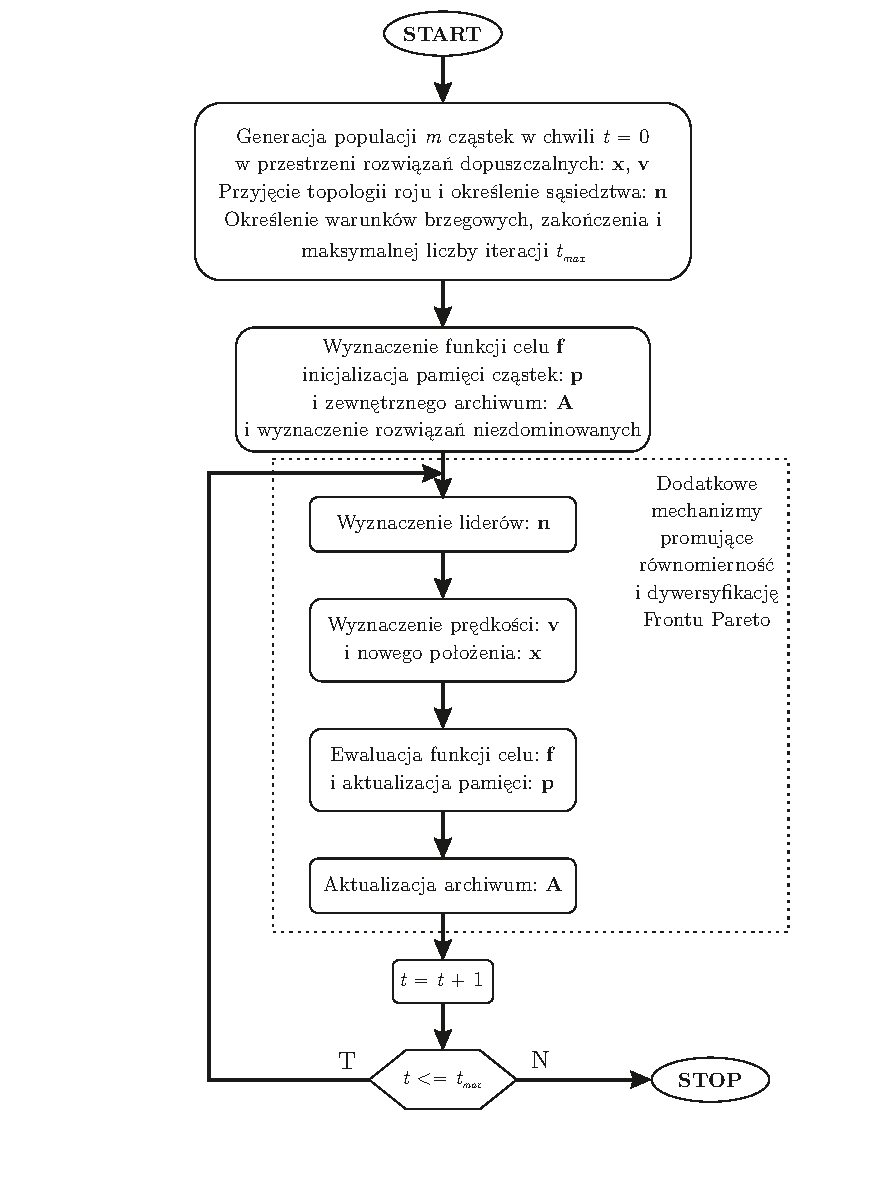
\includegraphics[trim= 50 20 20 0, clip,height=0.9\textheight]{/PSO/algorithm_multi/algoritm_multi.pdf}
	\captionsetup{justification=centering}
	\caption{Bazowy algorytm wielokryterialnej optymalizacji rojem cząstek (MOPSO)}
	\label{fig: pso_multi_algorithm}
\end{figure}

\clearpage

\subsection{Przykład teoretyczny}
Podobnie jak w przypadku wersji jednokryterialnej optymalizacji, wykonano przykład teoretyczny sprawdzający działanie zaimplementowanego algorytmu MOPSO. Jako wzorzec zaczerpnięto rozwiązanie problemu optymalizacji z pracy \parencite{Zavala2014}. Przedmiotem optymalizacji jest kratownica, składająca się z czterech prętów i obciążona jak na rysunku \ref{fig: pso_multi_testtruss}. Kratownica jest opisana na siatce kwadratowej o boku $L$. Problem optymalizacji opisany jest przez dwie funkcje celu: $f_1(\vect{x})$ - objętość materiału zastosowanego do budowy kratownicy i $f_2(\vect{x})$ - przemieszczenie węzła $A$ kratownicy pod obciążeniem zewnętrznym. Obie funkcje celu są minimalizowane. Wektor zmiennych projektowych stanowią pola przekrojów poszczególnych prętów $\vect{x}=[x_1,x_2,x_3,x_4]$. Parametry systemu stanowią: długość $L=200\,\text{cm}$, wartość obciążenia zewnętrznego $F=10\,\text{kN}$, moduł sprężystości materiału $E=2\cdot10^5\,\frac{\text{kN}}{\text{cm}^2}$ oraz maksymalne naprężenia dopuszczalne $\sigma=10\,\frac{\text{kN}}{\text{cm}^2}$.
\begin{figure}[hbt!]
	\centering
	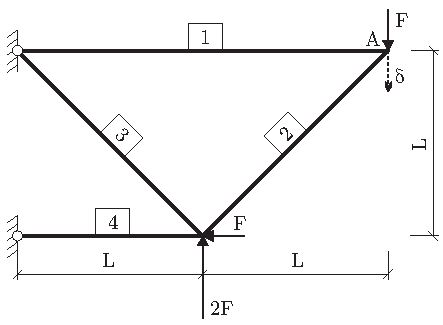
\includegraphics[width=0.60\linewidth]{/PSO/testkrata/truss_scheme.pdf} 
	\captionsetup{justification=centering}
	\caption{Schemat statyczny układu testowego optymalizacji wielokryterialnej}
	\label{fig: pso_multi_testtruss} 
\end{figure}




Wartość funkcji celu $f_1$ została obliczona wprost przez iloczyn pól przekrojów i długości prętów:
\begin{equation}
	f_1(\vect{x}) = L\cdot(2x_1+\sqrt{2}x_2+\sqrt{2}x_3+x_4)
\end{equation}

Aby uzależnić przemieszczenie węzła $A$ od zmiennych projektowych posłużono się zasadą prac wirtualnych. Wyznaczono rozkład sił wewnętrznych od obciążenia zewnętrznego i od obciążenia wirtualnego w miejscu badanego przemieszczenia (Rys. \ref{fig: pso_testtruss_results}). Następnie wyznaczono wartość przemieszczeń zgodnie z wzorem (\ref{eq: pso_test_truss_norma_forces}).

\begin{figure}[hbt!]
	\centering
	\subfloat[]{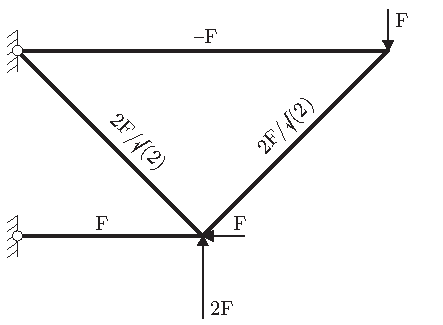
\includegraphics[width=0.5\linewidth]{/PSO/testkrata/truss_scheme_zew.pdf} \label{fig: pso_testtruss_zew}}
	\subfloat[]{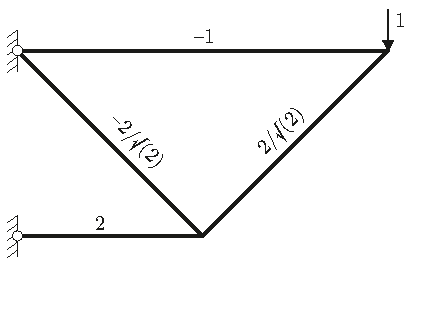
\includegraphics[width=0.5\linewidth]{/PSO/testkrata/truss_scheme_wew.pdf} \label{fig: pso_testtruss_wirt}}
	\captionsetup{justification=centering}
	\caption{Wartości sił normalnych w prętach kratownicy: (a) od obciążeń zewnętrznych, (b) od obciążenia wirtualnego}
	\label{fig: pso_testtruss_results}
\end{figure}

\begin{equation} \label{eq: pso_test_truss_norma_forces}
\begin{split}
	f_2(\vect{x}) =\delta= \sum_{n=1}^{4} \frac{N_i\bar{N}_i}{EA_i}L_i &=\frac{1}{E}\bigg(\frac{2FL}{x_1}+ \frac{4\sqrt{2}FL}{2x_2}- \frac{4\sqrt{2}FL}{2x_3}+\frac{2FL}{x_4}\bigg) \\
	&=\frac{2FL}{E}\bigg(\frac{1}{x_1}+\frac{\sqrt{2}}{x_2}-\frac{\sqrt{2}}{x_3}+\frac{1}{x_4}\bigg)
\end{split}
\end{equation}

\pagebreak[4]
Autorzy przykładu zaproponowali ograniczenie przestrzeni rozwiązań dopuszczalnych przez podanie dopuszczalnych maksymalnych i minimalnych naprężeń w prętach. Po przekształceniach ograniczenia dla zmiennych projektowych podano następujące:
\begin{equation}
	\begin{split}
	\frac{F}{\sigma} \le x_1,x_4 \le \frac{3F}{\sigma}\\
	\frac{\sqrt{2}F}{\sigma} \le x_2,x_3 \le \frac{3F}{\sigma}
	\end{split}
\end{equation}

Algorytm MOPSO oprogramowano w języku Python. Parametry prędkości PSO zostały przyjęte tak samo jak w punkcie \ref{sect: pso_single_teor_exampl}. Metodą z użyciem sekwencji Haltona wygenerowano populację 70 cząstek i wykonano 40 iteracji aktualizacji całej populacji. Z uwagi na niewymagające obliczeniowo funkcje celu, nie założono maksymalnej objętości zewnętrznego archiwum i zawyżono potencjalnie niezbędną liczbę wszystkich iteracji. Dodatkowo wszystkie wyliczone rozwiązania zapisano w bazie wszystkich dotychczasowych rozwiązań \teng{knowlagebase}. Wprowadzono modyfikację wyboru lidera roju, pozwalającą poprawić równomierność rozmieszczenia rozwiązań niezdominowanych. Mechanizm wzorowany był na pomiarze odległości pomiędzy cząstkami niezdominowanymi w przestrzeni wartości \parencite{Deb2002} i składał się z następujących kroków:
\begin{enumerate}
	\item Posortowanie rozwiązań przechowywanych w archiwum według jednej z funkcji celu.
	\item Normalizacja osi. Wyznaczenie różnicy pomiędzy największą, a najmniejszą wartością dla każdej funkcji celu oddzielnie. Następnie obliczenie ilorazu wartości danej funkcji celu przez odpowiadającą jej wyznaczoną różnicę.
	\item Wyznaczenie odległości w przestrzeni funkcji celu pomiędzy sąsiednimi cząstkami, posortowanymi według funkcji celu.
	\item Losowy wybór pomiędzy cząstkami cechującymi się największą wzajemną odległością.
\end{enumerate}
Normalizacja osi została dodana, ponieważ funkcje celu cechowały się innym rzędem wartości. Objętość materiału wyznaczana była w tysiącach, a przemieszczenie były mniejsze od jedności. Mimo zupełnie innego znaczenia powyższych liczb (inne jednostki), kiedy rozpatruje się odległości pomiędzy punktami wzdłuż Frontu Pareto, wartości dużo większe dominują nad mniejszymi. Przy stosowaniu mechanizmów opartych na pomiarze zagęszczenia i odległości zalecane jest takie zmodyfikowanie funkcji celu by wyznaczone wartości wszystkich funkcji celu były tego samego rzędu.

Na rysunku \ref{fig: pso_testkrata_all} zaprezentowano wizualizację przebiegu procesu optymalizacji MOPSO. Każdy z wykresów prezentuje stan rozwiązania po podanej pełnej iteracji $t$ zmiany położenia cząstek. Kolorem czarnym oznaczono aktualne położenie roju. Kolor czerwony pokazuje dotychczas znalezione rozwiązania niezdominowane - przybliżenie Frontu Pareto. Niebieskim punktem zaznaczono cząstkę pełniącą rolę lidera roju. Dodatkowo kolorem zielonym oznaczono historię wszystkich dotychczasowych rozwiązanych (knowlagebase). Rezultaty testu są zgodne z rozwiązaniem podanym w \parencite{Zavala2014}. Można również stwierdzić, że Front Pareto został odwzorowany równomiernie oraz dokładnie.


\begin{figure}[p]
	\centering
	\subfloat[$t=2$]{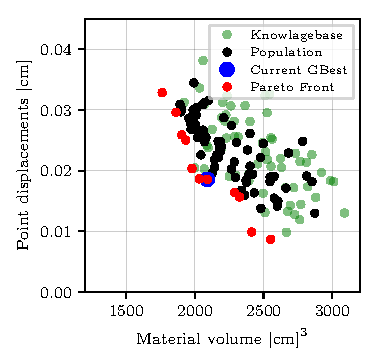
\includegraphics[trim=00 5 0 5, clip,height=0.2\textheight]{/PSO/testkrata/results/fig_02_98_2021-02-21_14_05_40.pdf}}
	\subfloat[$t=3$]{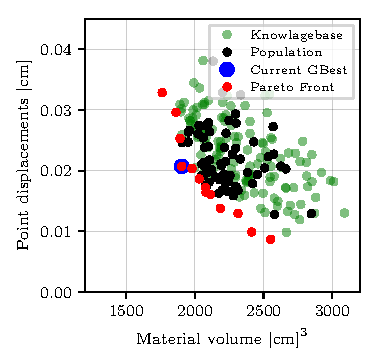
\includegraphics[trim=18 5 0 5, clip,height=0.2\textheight]{/PSO/testkrata/results/fig_03_98_2021-02-21_14_05_46.pdf}}
	\subfloat[$t=4$]{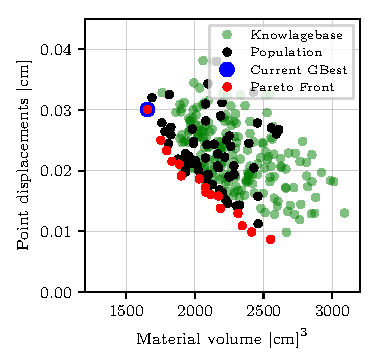
\includegraphics[trim=18 5 0 5, clip,height=0.2\textheight]{/PSO/testkrata/results/fig_04_98_2021-02-21_14_05_54.pdf}}\\
	\subfloat[$t=5$]{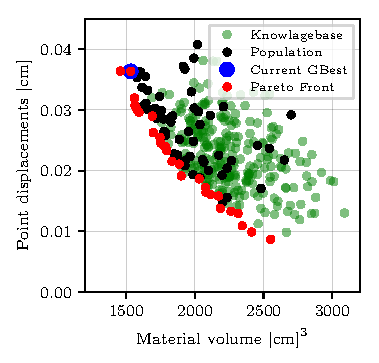
\includegraphics[trim=00 5 0 5, clip,height=0.2\textheight]{/PSO/testkrata/results/fig_05_98_2021-02-21_14_06_02.pdf}}
	\subfloat[$t=6$]{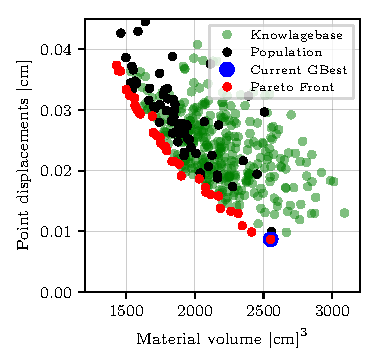
\includegraphics[trim=18 5 0 5, clip,height=0.2\textheight]{/PSO/testkrata/results/fig_06_98_2021-02-21_14_06_11.pdf}}
	\subfloat[$t=7$]{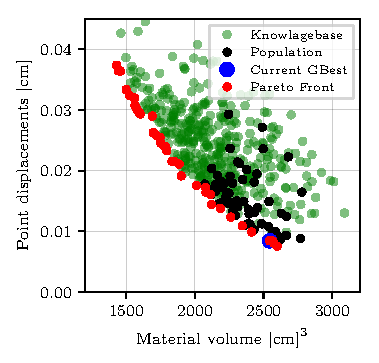
\includegraphics[trim=18 5 0 5, clip,height=0.2\textheight]{/PSO/testkrata/results/fig_07_98_2021-02-21_14_06_18.pdf}}\\
	\subfloat[$t=8$]{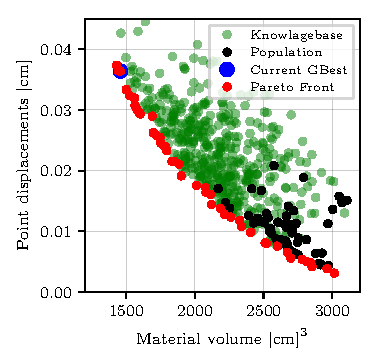
\includegraphics[trim=00 5 0 5, clip,height=0.2\textheight]{/PSO/testkrata/results/fig_08_98_2021-02-21_14_06_26.pdf}}
	\subfloat[$t=9$]{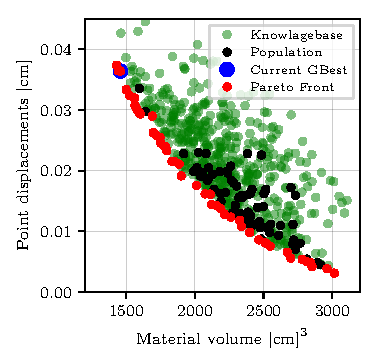
\includegraphics[trim=18 5 0 5, clip,height=0.2\textheight]{/PSO/testkrata/results/fig_09_98_2021-02-21_14_06_34.pdf}}
	\subfloat[$t=10$]{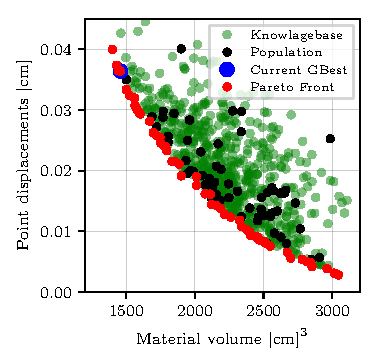
\includegraphics[trim=18 5 0 5, clip,height=0.2\textheight]{/PSO/testkrata/results/fig_10_98_2021-02-21_14_06_44.pdf}}\\
	\subfloat[$t=20$]{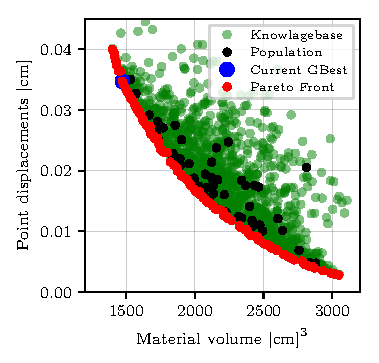
\includegraphics[trim=00 5 0 5, clip,height=0.2\textheight]{/PSO/testkrata/results/fig_20_98_2021-02-21_14_07_59.pdf}}
	\subfloat[$t=30$]{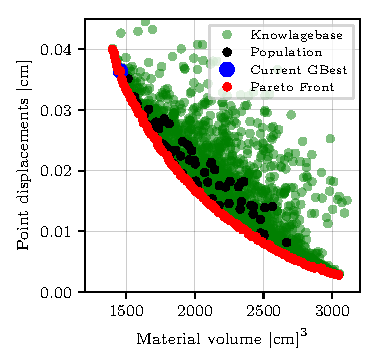
\includegraphics[trim=18 5 0 5, clip,height=0.2\textheight]{/PSO/testkrata/results/fig_30_98_2021-02-21_14_09_12.pdf}}
	\subfloat[$t=40$]{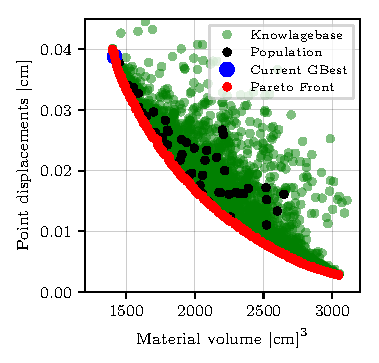
\includegraphics[trim=18 5 0 5, clip,height=0.2\textheight]{/PSO/testkrata/results/fig_41_98_2021-02-21_14_10_39.pdf}}\\
	\captionsetup{justification=centering}
	\caption{Etapy rozwiązania testowego problemu optymalizacji wielokryterialnej metodą roju cząstek (MOPSO)}
	\label{fig: pso_testkrata_all}
\end{figure}

%\vfill

%\pagebreak[4]
\section{Optymalizacja wspomagana uczeniem maszynowym}
Optymalizacja wielokryterialna korzystająca nawet z szybko zbiegających algorytmów wymaga najczęściej wielokrotnych ewaluacji funkcji celu. W przypadku rzeczywistych problemów inżynierskich wyznaczanie wartości funkcji celu często jest złożonym procesem, który wymaga długotrwałych symulacji numerycznych. Ostatecznie otrzymanie dobrej jakości Frontu Pareto może okazać się bardzo trudne, albo wręcz niemożliwe z uwagi na czas wymagany na rozwiązanie zadania. Generalnie stosowane są dwie ścieżki, które pozwalają poradzić sobie z tym problemem: zrównoleglenie obliczeń przez podział na podproblemy i zwiększenie efektywności algorytmu przez zatrudnienie surogatów \teng{surrogates} \parencite{Haftka2016}. Surogaci zdefiniowani są jako proste modele algebraiczne dopasowane do dotychczas wyznaczonych wartości funkcji i ograniczeń. Do przewidywania przybliżonego rozwiązania wykorzystywane są metody aproksymacji bazujące na Procesach Gaussowskich \teng{Gaussian Process (GP)} \parencite{Rasmussen2006,Rasmussen2010}. Opierają się one na zbudowaniu bazy rozwiązań, na podstawie której algorytm uczy się i jest w stanie przewidywać wyniki bez standardowej ewaluacji funkcji celu. Każda funkcja celu jest modelowana niezależnie, a algorytm dostarcza wartość funkcji oraz miarę niepewności tego rozwiązania dla nowych zmiennych projektowych. 
W kontekście optymalizacji rojem cząstek, przewidywane rozwiązania mogą być ocenione jako prawdopodobnie należące do frontu Pareto i zostać zaproponowane jako kandydaci do wyznaczenia funkcji celu w kolejnych iteracjach. Przykłady takiego podejścia pokazują metody: Pareto Active Learning (PAL) \parencite{Zuluaga2013} i w wersji rozbudowanej $\epsilon$-Pareto Active Learning ($\epsilon$-PAL) \parencite{Zuluaga2016} oraz Active Learning of Pareto Front (ALP) \parencite{Campigotto2013}. W pracach \cite{Lv2017,Lv2019} zaproponowano algorytm optymalizacji wielokryterialnej oparty na PSO i technice $\epsilon$-PAL: Multi-Objective Particle Swarm Algorithm (MOPSAL). Takie podejście potrafi znacząco ograniczyć liczbę obliczeń funkcji celu i przyspieszyć optymalizację wymagających problemów nawet o 70\% \parencite{Zuluaga2016}.



